\chapter{Vecteurs - partie 1}
\thispagestyle{fancy}

\section{Définitions et propriété}

\subsection{Norme d'un vecteur}

    \begin{bdefi}
        \begin{spacing}{1.6}
        	\dotfill \\
        	\pointille[\textwidth]
        \end{spacing}
    \end{bdefi}
    
\subsection{Produit scalaire}
    \begin{bdefi}
        \begin{minipage}[b]{0.65\linewidth}
            Soit $\vv{u}$ et $\vv{v}$ deux vecteurs du plan.\\
            On appelle \grasInDef{produit scalaire} de $\vv{u}$ par $\vv{v}$, noté $\vv{u}\cdot \vv{v}$, le nombre réel défini par :\\
            \begin{spacing}{1.6}
            \begin{itemDef}
                \item \pointille[\textwidth-0.3cm]
                \item \pointille[\textwidth-0.3cm]
            \end{itemDef}
        	\end{spacing}
        \end{minipage}\hfill
        \begin{minipage}[b]{0.3\linewidth}
        \begin{center}
            \newrgbcolor{qqwuqq}{0. 0.39215686274509803 0.}
            \psset{xunit=1cm,yunit=1cm,algebraic=true,dimen=middle,dotstyle=o,dotsize=5pt 0,linewidth=1.6pt,arrowsize=3pt 2,arrowinset=0.25}
            \begin{pspicture*}(1.3,0.8)(8.3,4.6)
            \psline[linewidth=1.2pt]{->}(2.,2.)(6.,2.)
            \psline[linewidth=1.2pt]{->}(2.,2.)(4.,4.)
            \rput[tl](3.7,1.8){\Large $\vv u$}
            \rput[tl](2.5,3.6){\Large $\vv v$}
            \pscustom[linewidth=1.2pt,linecolor=qqwuqq]{
\parametricplot{0.0}{0.78}{0.68*cos(t)+2.|0.68*sin(t)+2.}
\lineto(2.,2.)\closepath}
            \begin{scriptsize}
            \psdots[dotsize=5pt 0,dotstyle=*](2.,2.)
            \rput[bl](1.3,2.0){\Large $A$}
            \psdots[dotsize=5pt 0,dotstyle=*](6.,2.)
            \rput[bl](6.2,2.0){\Large $B$}
            \psdots[dotsize=5pt 0,dotstyle=*](4.,4.)
            \rput[bl](4.2,4.0){\Large $C$}
            \end{scriptsize}
            \end{pspicture*}
        \end{center}
        \end{minipage}
    \end{bdefi}
    
    \begin{brmqs}
        \begin{itemRem}
            \item $\vv{u}\cdot \vv{v}$ se lit $\vv{u}$ scalaire $\vv{v}$
            \item 	Si $\vv{AB}$ et $\vv{AC}$ sont deux représentants des vecteurs non nuls $\vv{u}$ et $\vv{v}$ alors :\\
            $\vv{u}\cdot \vv{v} = \vv{AB}\cdot \vv{AC} = \normeB{AB}\times\normeB{AC}\times\cos{(\widehat{BAC})}$
            \item 	\grasInRem{Attention} : Le produit scalaire de deux vecteurs est un nombre réel. Écrire par exemple $\vv{u}\cdot \vv{v}=\vv{0}$ est une maladresse à éviter !
        \end{itemRem}
    \end{brmqs}
    
    \begin{bmethodet}{calculer un produit scalaire}
        \grasInMet{Enoncé :} Calculer : $\vv{AB}\cdot \vv{AC}$ sachant que $AB=5$, $AC=4\sqrt{2}$ et $(\vv{AB},\vv{AC})=\dfrac{\pi}{4}$\\
        
    \end{bmethodet}
    
    \begin{bmethodet}{Calculer un produit scalaire à l'aide du cosinus}
        \grasInMet{Enoncé :} \\
        Soit un triangle équilatéral ABC de côté $a$. Calculer, en fonction de a, le produit scalaire $\vv{A B} \cdot \vv{A C}$.
        \begin{center}
            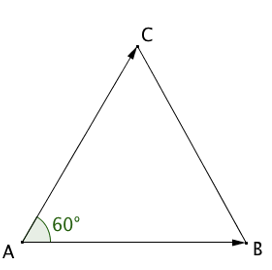
\includegraphics[scale=0.7]{1.04.IMG-01}
        \end{center}
        
    \end{bmethodet}
    
    \subsection{Propriété de symétrie du produit scalaire}
    
    \begin{bprop}
        Pour tout vecteur $\vv{u}$ et $\vv{v}$, on a : \dotfill 
    \end{bprop}
    
    \begin{bdemo}
    \end{bdemo}
    
    \subsection{opérations sur les produits scalaires}
    
    \begin{bprop}
        Pour tout vecteur $\vv{u}$,$\vv{v}$ et $\vv{w}$, on a :
        \begin{spacing}{1.6}
        	\begin{enumProp}
        		\item \pointille[\textwidth-1cm]
        		\item \pointille[\textwidth-1cm]
        	\end{enumProp}
        \end{spacing}
    \end{bprop}

    \subsection{Identités remarquables}
    
    \begin{bprop}
        Pour tout vecteur $\vv{u}$ et $\vv{v}$, on a :
        \begin{spacing}{1.6}
        \begin{enumProp}
        	\item \pointille[\textwidth-1cm]
        	\item \pointille[\textwidth-1cm]
        	\item \pointille[\textwidth-1cm]
        \end{enumProp}
    \end{spacing}
    \end{bprop}
    
    \begin{bdemot}{2ème formule : }
    	
    \end{bdemot}
    
       \section{Produit scalaire et orthogonalité}
    
    \subsection{Vecteurs orthogonaux}
    
    \begin{bprop}
        \begin{spacing}{1.6}
        	\dotfill 
        \end{spacing}
    \end{bprop}
    
    \begin{bdemo}
    \end{bdemo}
    
    \subsection{Projection orthogonale}
    
    \begin{bdefi}
         \begin{spacing}{1.6}
        	\dotfill \\
        	\pointille[\textwidth]
        	\pointille[\textwidth]
        \end{spacing}
        \begin{center}
            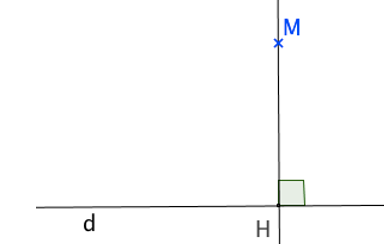
\includegraphics[scale=0.6]{1.04.IMG-04}
        \end{center}
    \end{bdefi}
    
    \begin{bprop}
        Soit $\vec{u}$ et $\vec{v}$ deux vecteurs non nuls du plan tels que $\vec{u}=\vv{O A}$ et $\vec{v}=\vv{O B}$.\\
        H est le projeté orthogonal du point $B$ sur la droite (OA). On a \dotfill
        \begin{center}
            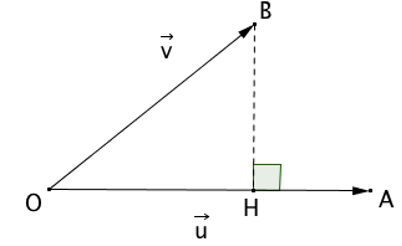
\includegraphics[scale=0.6]{1.04.IMG-06}
        \end{center}
    \end{bprop}
    
    \begin{bdemo}
    \end{bdemo}
    
    \begin{bmethodet}{Calculer un produit scalaire par projection}
        \grasInMet{Enoncé :}\\
        Soit un carré ABCD de côté $c$. Calculer, en fonction de $c,$ les produits scalaires:
        \begin{center}
            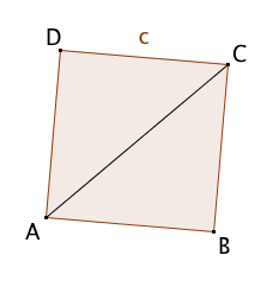
\includegraphics[scale=0.8]{1.04.IMG-07}
        \end{center}
        \begin{multicols}{3}
            \begin{enumMet}
                \item $\vv{A B} \cdot \vv{A C}$
                \item $\vv{A B} \cdot \vv{A D}$
                \item $\vv{A D} \cdot \vv{C B}$
            \end{enumMet}
        \end{multicols}
        
        \grasInMet{Réponse :}
    \end{bmethodet}
    
%    \subsection{Transformation de l'expression $\protect\vv{MA}\cdot\protect\vv{MB}$}
%    
%    \begin{propriete}
%        L'ensemble des points $\mathrm{M}$ vérifiant l'égalité $\vv{M A} . \vv{M B}=0$ est le cercle de diamètre [AB].
%    \end{propriete}
%    
%    \begin{demonstration}
%        \begin{center}
%            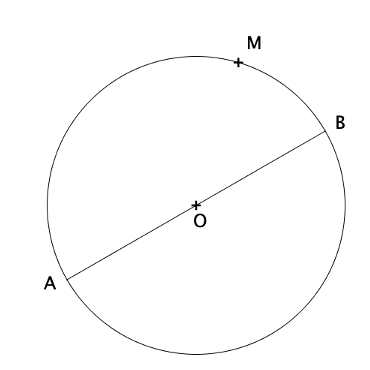
\includegraphics[scale=0.8]{1.04.IMG-08}
%        \end{center}
%        Soit O le milieu du segment [AB]. On a \\
%        $\vv{MA}\cdot \vv{MB}=0$\\
%        $\Leftrightarrow(\vv{M O}+\vv{O A}) \cdot(\vv{M O}+\vv{O B})=0$\\
%        Comme $\mathrm{O}$ est le milieu de $[\mathrm{AB}],$ on $\mathrm{a}: \vv{O B}=-\vv{O A}$ Soit:\\
%        $(M O+\vv{O A}) \cdot(\vv{M O}-\vv{O A})=0$\\
%        $\Leftrightarrow \vv{M O}^{2}-\vv{O A}^{2}=0 \quad \operatorname{car}(\vec{u}+\vec{v}) \cdot(\vec{u}-\vec{v})=\vec{u}^{2}-\vec{v}^{2}$\\
%        $\Leftrightarrow M O^{2}-O A^{2}=0$\\
%        Soit : $M O^{2}=O A^{2}$ soit encore $M O=O A$. M appartient donc au cercle de centre O et de rayon OA, c'est-à-dire le cercle de diamètre [AB].
%    \end{demonstration}
%    
%    \begin{propriete}
%        Un point M, distinct de A et B, appartient au cercle de diamètre [AB] si et seulement si le triangle ABM est rectangle en M.
%    \end{propriete}
%    
%    \begin{remarque}
%        Justification: $\vv{M A} \cdot \vv{M B}=0$ si et seulement si les vecteurs $\vv{M A}$ et $\vv{M B}$ sont orthogonaux.
%        \begin{center}
%            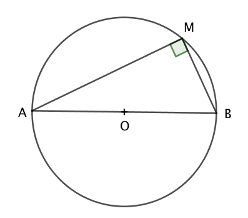
\includegraphics[scale=1]{1.04.IMG-09}
%        \end{center}
%    \end{remarque}
    
    \section{Produit scalaire dans un repère orthonormé}
    
    Le plan est muni d'un repère orthonormé \Rij
    
    \begin{bprop}
        Soit $\vec{u}$ et $\vec{v}$ deux vecteurs de coordonnées respectives $\Coord{u}{x}{y}$ et $\Coord{v}{x'}{y'}$. On a: \dotfill
    \end{bprop}
    
    \begin{bdemo}
    \end{bdemo}
    
    \begin{bmethodet}{Calculer un produit scalaire à l'aide des coordonnées}
        \grasInMet{Enoncé :}\\
        Soit $\Coord{u}{5}{-4}$ et $\Coord{v}{-3}{7}$ deux vecteurs.\\
        Calculer $\vec{u} \cdot \vec{v}$
        \ \\
        \grasInMet{Réponse :}\\
    \end{bmethodet}


    \begin{bmethodet}{Déterminer un angle à l'aide du produit scalaire}
    	\begin{minipage}{0.65\linewidth}
    		\grasInMet{Enoncé :}\\
    		Calculer la mesure de l'angle $(\vv{A B} ; \vv{C D})$ en lisant les coordonnées des points $\mathrm{A}, \mathrm{B}, \mathrm{C}$ et $\mathrm{D}$ dans le repère.\\
    		
    		\ \\
    		\grasInMet{Réponse :}\\
    	\end{minipage} \hfill
    	\begin{minipage}{0.35\linewidth}
    		\begin{center}
    			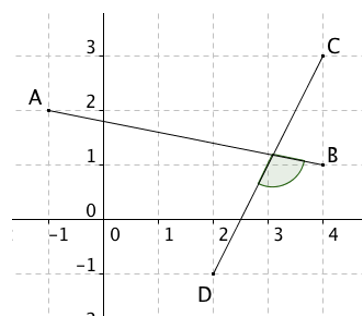
\includegraphics[scale=0.7]{1.04.IMG-10}
    		\end{center}
    	\end{minipage}
        
    \end{bmethodet}
    
    % \section{Produit scalaire et norme}
    
    % \subsection{Propriétés}

    % Soit un vecteur $\vec{u},$ on a :
    % $\vec{u} \cdot \vec{u}=\|\vec{u}\| \times\|\vec{u}\| \times \cos (\vec{u} ; \vec{u})=\|\vec{u}\|^{2} \times \cos 0=\|\vec{u}\|^{2}$\\
    % et\\
    % $\vec{u}\cdot \vec{u}=\vec{u}^{2}$\\
    % On a ainsi $: \vec{u}^{2}=\vec{u} \cdot \vec{u}=\|\vec{u}\|^{2}$
    
    % \begin{propriete}
    %     Propriété : Soit $\vec{u}$ et $\vec{v}$ deux vecteurs. On a :
    %     \begin{itemDef}
    %         \item $\vec{u} \cdot \vec{v}=\dfrac{1}{2}\left(\|\vec{u}\|^{2}+\|\vec{u}\|^{2}-\|\vec{u}-\vec{v}\|^{2}\right)$
    %         \item $\vec{u} \cdot \vec{v}=\dfrac{1}{2}\left(\|\vec{u}+\vec{v}\|^{2}-\|\vec{u}\|^{2}-\|\vec{v}\|^{2}\right)$
    %         \item $\vec{u} \cdot \vec{v}=\dfrac{1}{4}\left(\|\vec{u}+\vec{v}\|^{2}-\|\vec{u}-\vec{v}\|^{2}\right)$
    %     \end{itemDef}
    % \end{propriete}
    
    % \begin{demonstrationTitre}{Démonstration de la première formule}
    %     \begin{align*}
    %         \|\vec{u}-\vec{v}\|^{2}&=(\vec{u}-\vec{v})^{2} \\
    %         &=\vec{u}^{2}-2 \vec{u} \cdot \vec{v}+\vec{v}^{2} \\
    %         &=\|\vec{u}\|^{2}-2 \vec{u} \cdot \vec{v}+\|\vec{v}\|^{2}
    %     \end{align*}
    %     Donc $\vec{u} \cdot \vec{v}=\dfrac{1}{2}\left(\|\vec{u}\|^{2}+\|\vec{u}\|^{2}-\|\vec{u}-\vec{v}\|^{2}\right)$
    % \end{demonstrationTitre}

    % \begin{propriete}
    %     Soit $A, B$ et $C$ trois points du plan. On a :
    %     $\vv{A B} \cdot \vv{A C}=\dfrac{1}{2}\left(A B^{2}+A C^{2}-B C^{2}\right)$
    % \end{propriete}
    
    % \begin{demonstration}
    %     \begin{align*}
    %         \vv{A B} \cdot \vv{A C}&=\dfrac{1}{2}\left(\|\vv{A B}\|^{2}+\|\vv{A C}\|^{2}-\|\vv{A B}-\vv{A C}\|^{2}\right) \\
    %         &=\dfrac{1}{2}\left(A B^{2}+A C^{2}-\|\vv{C B}\|^{2}\right) \\
    %         &=\dfrac{1}{2}\left(A B^{2}+A C^{2}-B C^{2}\right)
    %     \end{align*}
    % \end{demonstration}
    
    % \begin{exemple}
    %     Si $\mathrm{AB}=6, \mathrm{AC}=5$ et $\mathrm{CB}=4$ alors:
    %     $$
    %     \vv{A B} \cdot \vv{A C}=\frac{1}{2}\left(A B^{2}+A C^{2}-C B^{2}\right)=\frac{1}{2}\left(6^{2}+5^{2}-4^{2}\right)=\frac{1}{2}(36+25-16)=\frac{45}{2}
    %     $$
    % \end{exemple}
    
    % \begin{methodeTitre}{Calculer un produit scalaire à l'aide des normes}
    %     \grasInMet{Enoncé :}\\
    %     On considère la figure ci-dessous, calculer le produit scalaire $\vv{C G} \cdot \vv{C F}$
    %     \begin{center}
    %         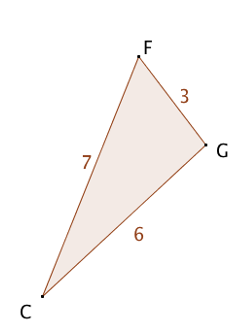
\includegraphics[scale=0.8]{1.04.IMG-02}
    %     \end{center}
    %     \ \\
    %     \grasInMet{Réponse :}\\
    %     $\vv{C G} \cdot \vv{C F}=\frac{1}{2}\left(C G^{2}+C F^{2}-G F^{2}\right)$\\
    %     $=\dfrac{1}{2}\left(6^{2}+7^{2}-3^{2}\right)$\\
    %     $=38$
    % \end{methodeTitre}
    
    % \subsection{Théorème d'Al Kashi}
    
    % \begin{theoreme}
    %     Dans un triangle $\mathrm{ABC},$ on a, avec les notations de la figure :
    %     $$
    %     a^{2}=b^{2}+c^{2}-2 b c \cos \hat{A}
    %     $$
    %     \begin{center}
    %         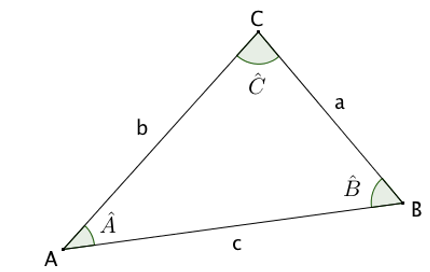
\includegraphics[scale=0.8]{1.04.IMG-03}
    %     \end{center}
    % \end{theoreme}
    
    % \begin{demonstration}
    %     $\vv{A B} \cdot \vv{A C}=A B \times A C \times \cos \hat{A}=b c \cos \hat{A}$\\
    %     et\\
    %     $\vv{A B} \cdot \vv{A C}=\frac{1}{2}\left(A B^{2}+A C^{2}-B C^{2}\right)=\frac{1}{2}\left(b^{2}+c^{2}-a^{2}\right)$\\
    %     Donc $: \frac{1}{2}\left(b^{2}+c^{2}-a^{2}\right)=b c \cos \hat{A}$\\
    %     Soit $: b^{2}+c^{2}-a^{2}=2 b c \cos \hat{A}$\\
    %     Soit encore $: a^{2}=b^{2}+c^{2}-2 b c \cos \hat{A}$\\
    % \end{demonstration}
    
    % \begin{methodeTitre}{Calculer un produit scalaire à l'aide des normes}
    %     \grasInMet{Enoncé :}\\
    %     On considère la figure ci-dessous, calculer la mesure de l'angle $\widehat{B A C}$ au degré près.
    %     \begin{center}
    %         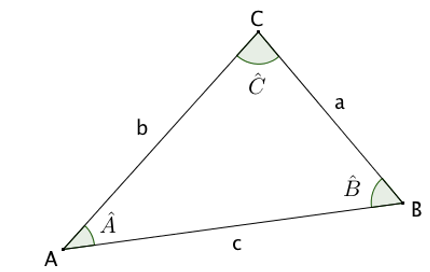
\includegraphics[scale=0.8]{1.04.IMG-03}
    %     \end{center}
    %     \ \\
    %     \grasInMet{Réponse :}\\
    %     D'après le théorème d'Al Kashi, on a :\\
    %     $C B^{2}=A B^{2}+A C^{2}-2 \times A B \times A C \times \cos \widehat{B A C}$\\
    %     $4^{2}=6^{2}+5^{2}-2 \times 6 \times 5 \times \cos \widehat{B A C}$\\
    %     $16=36+25-60 \cos \widehat{B A C}$\\
    %     $60 \cos \widehat{B A C}=36+25-16$\\
    %     $60 \cos \widehat{B A C}=45$\\
    %     $\cos \widehat{B A C}=\dfrac{45}{60}$\\
    %     $\cos \widehat{B A C}=\dfrac{3}{4}$\\
    %     $\widehat{B A C} \approx 41^{\circ}$
    % \end{methodeTitre}
    
    % \section{Vecteur Normal}
    
    % \subsection{définition et propriétés}
    
    % \begin{definition}
    %     Un \grasInDef{vecteur normal} à une droite $d$ quelconque du plan est un vecteur non nul et orthogonal à un vecteur directeur de $d$.
    % \end{definition}
    
    % \begin{propriete}
    %     Deux droites du plan sont perpendiculaires si et seulement si un vecteur normal de l'une est orthogonal à un vecteur normal de l'autre.
    % \end{propriete}
    
    % \begin{demonstration}
    %     On suppose que $d$ et $d^{\prime}$ sont perpendiculaires. Si $\vec{u}$ est un vecteur directeur de $d$ et $\vec{v}$ de $d^{\prime},$ alors $\vec{u}$ et $\vec{v}$ sont orthogonaux. $\vec{v}$ étant normal à $d$ et $\vec{u}$ à $d^{\prime},$ la propriété est vérifiée.\\
    %     Réciproquement, si $\vec{u},$ vecteur normal à $d,$ est orthogonal à $\vec{v},$ vecteur normal à $d^{\prime},$ alors $\vec{v}$ est un vecteur directeur de $d$ et $\vec{u}$ de $d^{\prime} .$ Ayant des vecteurs directeurs orthogonaux, d et $d^{\prime}$ sont perpendiculaires.
    % \end{demonstration}
    
    % \begin{methode}
    %     \grasInMet{Enoncé:}\\
    %     Soit $d$ une droite de vecteur directeur $\Coord{u}{3}{5}$.
    %     \begin{enumMet}
    %         \item Déterminer une condition sur les coordonnées d'un vecteur $\vv{n}$ non nul pour qu'il soit normal à $d$.
    %         \item Le vecteur $\Coord{v}{-10}{6}$ est-il un vecteur normal à $d$?
    %     \end{enumMet}
        
    %     \grasInMet{Réponse:}\\
    %     \begin{enumMet}
    %         \item Si $\Coord{n}{x}{y}$ est un vecteur normal à $d$, alors il est orthogonal à $\vv{u}$.\\
    %         Donc $\vv{u} \cdot \vv{n}=3 x+5 y=0$ soit $y=-\dfrac{3}{5} x$.\\
    %         Les coordonnées de $\vv{n}$ sont donc de la forme $\CoordSV{x}{-\dfrac{3}{5}x}$ avec $x \in \R$.
    %         \item On calcule le produit scalaire $\vv{u}\cdot\vv{v}$\\
    %         $\vv{u}\cdot\vv{v}=3\times(-10)+5\times6=-30+30=0$\\
    %         le vecteur $\vv{v}$ est orthogonal au vecteur directeur $\vv{u}$ de la droite $d$, donc $\vv{v}$ est un vecteur normal à $d$. 
    %     \end{enumMet}
    % \end{methode}
    
    % \subsection{Équations cartésiennes et vecteur normal}
    
    % \begin{proprieteTitre}{Rappel : équations cartésiennes}
    %     Toute droite $D$ admet une équation de la forme $a x+b y+c=0$ avec $(a ; b) \neq(0 ; 0) .$ Un \grasInDef{vecteur directeur} de $D$ est $\Coord{u}{-b}{a}$ \\
    %     Cette équation est appelée \grasInDef{équation cartésienne} de la droite $D$.
    % \end{proprieteTitre}
        
    % \begin{propriete}
    %     Soient $a, b$ et $c$ trois réels tels que $a$ et $b$ ne sont pas simultanément nuls.\\
    %     La droite d'équation cartésienne $a x+b y+c=0$ admet pour \grasInDef{vecteur normal} le vecteur $\Coord{n}{a}{b}$.\\
    %     \ \\
    %     Réciproquement, toute droite ayant pour \grasInDef{vecteur normal} le vecteur non nul $\Coord{n}{a}{b}$ admet une équation cartésienne de la forme $a x+b y+c=0$.
    % \end{propriete}
        
    % \begin{exemple}
    %     La droite d'équation cartésienne $3 x-4 y+5=0$ admet pour vecteur normal le vecteur $\Coord{n}{3}{-4}$  et pour vecteur directeur le vecteur $\Coord{u}{4}{3}$.\\
    %     On a bien $\vv{n} \cdot \vv{u}=0$
    % \end{exemple}
    
    % \begin{methode}
    %     \grasInMet{Enoncé:}\\
    %     Dans un repère orthonormé, déterminer, de deux façons différentes, une équation cartésienne de la droite $d$ passant par le point $\mathrm{A}(5 ;-1)$ et de vecteur normal $\Coord{n}{2}{-3}$.
        
    %     \grasInMet{Réponse:}\\
    %     \begin{enumMet}
    %         \item 1. On lit sur le vecteur normal que $a=2$ et $b=-3$.
    %         Donc une équation de $d$ est de la forme $2 x-3 y+c=0$. $\mathrm{A}(5 ;-1) \in d$ donc $2 \times 5-3 \times(-1)+c=0$ et donc $c=-13$.\\
    %         Ainsi, une équation de la droite $d$ est $2 x-3 y-13=0$.
    %         \item Soit $\mathrm{M}(x ;y)$ appartenant à $d .$ Alors $\vv{\mathrm{AM}}$ est un vecteur directeur de $d$ et est orthogonal au vecteur $\vv{n}$.\\
    %         $\vv{\mathrm{AM}} \cdot \vv{n}=0 \iff \CoordSV{x-5}{y+1} \cdot \CoordSV{2}{-3}=0 \iff 2(x-5)-3(y+1)=0 \iff 2 x-3 y-13=0$\\
    %         Donc une équation de la droite $d$ est $2 x-3 y-13=0$
    %     \end{enumMet}
    % \end{methode}

